\chapter{Measure detector}\label{chap:measure-detector}

In this chapter we will lay out the work that was done for the measure detector. First we will cover the general structure of music scores and the assumptions made that follow from that structure. After that we will cover the implementation of the measure detector, followed by the evaluation of results with both existing datasets and the data collected as described in Chapter \ref{chap:data-description}.

\section{Music scores}\label{sec:measure-detector-music-scores}

\begin{wrapfigure}{R}{0.5\textwidth}
    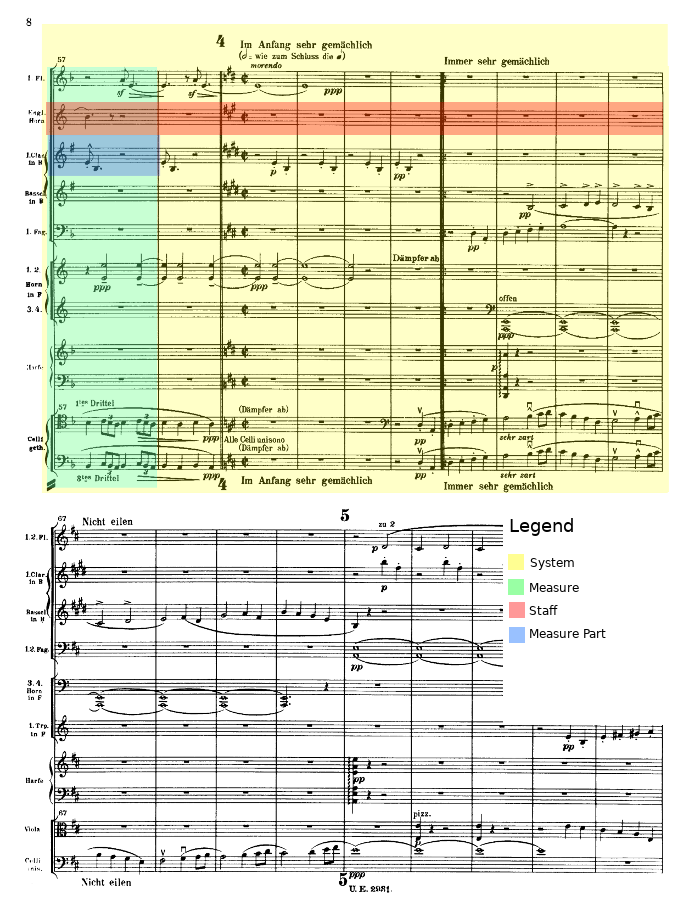
\includegraphics[width=0.5\textwidth]{images/score-structure.png}
    \centering
    \caption{Example structure of a page of music}
    \label{fig:page-structure}
\end{wrapfigure}

To understand the steps that need to be taken when implementing a measure detector, we first describe the general structure of a music score in this section. Each page of a music score contains one or more sytems. A system can be defined as an excerpt of a full page, having all the voices or instruments synchronized in time. A system will span the total width of the page, minus page margins, and subsequent systems will be put one beneath the other, continuing on subsequent pages depending on space. Each system can be seen as a grid of voices and measures. The rows of this grid represent the voices, each voice has a single staff, and the columns represent the measures. Each cell in this grid we then define as an individual measure. Terminology on this can get a little ambiguous, since in general music practise the term measure is used interchangably for both columns and cells in this grid, since generally musicians will mostly work with individual parts instead of the whole score, which unifies both these concepts since the columns in these individual parts are only of size 1. For clarity from now on we will refer to the columns as system measures and to the cells as measures, since this is done in the literature as well (e.g. \citep{Zalkow2019}). An example of such a structure is given in Figure \ref{fig:page-structure}, where a system, staff, measure and individual measure are outlined on a page of music. From this example it is already clear that there is more content on a page of music than just this grid, but for our purposes, the definition as given above should suffice.

Note that although it frequently occurs that different instruments or voices share a staff, this only makes a semantic difference, not a syntactical one. The purpose of this measure detector is to find the syntax of the music only, having a single voice versus multiple voices in a single staff can only change a staff rom containing monophonic to polyphonic contents, but this difference does not influence the measure detector, since it is expected to be able to handle polyphonic contents anyways, since polyphonic instruments also frequently occur in music scores.

\section{Detecting the grid}\label{sec:measure-detector-detecting}
This general structure of a page as layed out above will be used to detect the positions of the rows and columns of this grid on a page of music. Before any segmentation is done, some preprocessing is performed on the page. First we use morphology operations to find profiles of the vertical and horizontal line segments on the page. Using the horizontal profile, any rotation in the page that might have occurred due to scanning of the original score is rectified. Next the rotated page is inverted, making it white on black, thresholded by using Otso thresholding \citeneeded and then Gaussian blur is applied to smooth out some noise. The detection steps will be performed on the resulting image, complemented by the obtained profiles for vertical and horizontal line segments.

The first step of detection is done at the system level. There is a high level of separation between systems on a page, there are no connected components between them, which allows for segmentation through binary propagation. This binary propagation step will fill in each of the systems, allowing for easy detection of a few large blocks on the page, each of which is a candidate to be a system. A candidate system is only considered to be a system if there are horizontal and vertical lines detected in that system, this is to filter out extraneous parts on the page such as titles and text. From here on, in each system the vertical and horizontal profiles are used to detect the columns and rows in the system. First the staffs are detected by using the SciPy peak detection algorithm \citeneeded on the cutout of the horizontal profile containing only the current system in question. The detected peaks are grouped based on individual distance; if a next peak is further away twice the mean distance between peaks, a new grouping is created. These groupings are considered to be staffs in the system. This method is prefered over simply grouping five concurrent peaks together, which could also be an option considering common western music notation generally uses staffs consisting of five lines. However, this does not always hold true, percussion instruments for example can be notated with single lines only, and noise on a page might cause the peak detection algorithm to miss out on a line, making the results incorrect as well. With the staffs detected, the measures are now found using a similar method. Peak detection is performed on the cutout of the vertical profile, again containing only the current system, but removing the information contained within the boundaries of the previously detected staffs. Since we are detecting vertical lines, there is the possibility that note staffs are detected as well. Especially when a large part of the ensemble plays a note at the same time, this can yield a false positive while trying to find the measure boundaries. Therefore the information contained within the staffs, where most of the note staffs can be found, is removed. Since the barlines span the entire hight of the system, these can still be detected, even though some of that information is also removed. Now that the rows and columns of the grid are detected, the individual measures are simply found at the intersection. Note however that horizontally there is empty space between the boundaries of staffs. This is considered disputed teritory. Notes, accidentals and other markings of both the above and below staffs are allowed to spill over in this space, therefore there is no straight forward way to determine which part of this space belongs to which staff, that division is in a lot of cases non-linear. How this is handled can differ between applications of this detector, therefore no fixed solution is given here, however two imperfect possibilities are given here. Both of them suffer from the fact that they try a linear division, which is not always a possibility.

\subsection{Smallest intersection method}
The smallest intersection method works in two parts: first a set of baselines per system are established, and then these baselines are corrected for each individual block in that system. The baselines are established from the vertical intensity profile of the system. Each of the bars consist of 5 small peaks, corresponding to the 5 lines in a bar. These 5 peaks grouped together can be detected as one broader peak. The baselines are set as the middle points between each of these detected peaks. Next the baselines are corrected on a per block basis. This second step is necessary, since in the scores it can occur that notes and related annotations can cross an established baseline into the “territory” of measures above or below it. This crossing over can change per block, and therefore a correction per block is necessary. This second step finds within a predefined distance from the baseline the points with the lowest value in the intensity profile. These points indicate that when segmenting at these points, the least amount of information, indicated by white pixels, will be segmented, and therefore these points should be considered as good segmenting points. When finding these candidate points a small margin from the minimum intensity value is taken, and the point closest to the baseline is chosen as the segmenting point.

\subsection{Largest region method}
The largest region method divides the region in between two peaks into regions, where regions are separated from each other by intensity values above a certain threshold. The largest of these regions is taken, as this indicated the largest part between two measures where there is little to no information. The middle of this region is chosen as the segmenting point. In Figure 3 two examples are given of segmented pages using the image processing approach with the largest region method.

Figure 3: Two examples of score pages segmented with the largest region method.    
Evaluation
The drawback of this image processing method is that performance of the segmenter is hard to evaluate. The CNN based method had in this respect the advantage of having annotated examples. Unfortunately, these examples are not applicable to evaluation of the image processing approach, since that segments a level deeper; where the CNN approach segments at the block level, the image processing approach segments at the measure level. Currently evaluation has to be done by hand because of the lack of a corpus of segmented music scores. A tool is under development that can hopefully make this process more efficient and over time can hopefully help to create a corpus of segmented measures.

